%% ------------------------------------------------------------------------- %%
\chapter{Trabalhos Relacionados}

\noindent Neste capítulo serão apresentadas as principais ferramentas para abertura e encaminhamento de solicitação de ordem de serviço atualmente em produção, apontando suas principais características e pontos positivos além de expor as limitações encontradas. Em sequência, será apresentado uma visão geral sobre os mais recentes casos de estudo da aplicação do \acrshort{itil} na literatura, expondo os diversos benefícios de sua adoção.

\section{Aplicativos}

\noindent Atualmente, estão disponíveis diversas aplicações \textit{web} e \textit{mobile} no mercado que resolvem o problema de gerenciamento de ordens de serviço. No município de Palmas está em execução o aplicativo Alô Pequi \cite{alo_pequi}, inciativa da prefeitura de Palmas que possui como objetivo atender a necessidade do cidadão palmense em apontar os problemas de infraestrutura da cidade. No país existem diversas soluções para o problema mas a que se destaca de maneira acentuada é a plataforma Colab \cite{colab} pois contém aproximadamente mais de 50 mil \textit{downloads} na plataforma de aplicativos \textit{Google Play}. Seu diferencial está no modelo de rede social de colaboração como proposta do aplicativo. As próximas seções trazem uma visão geral das soluções atuais, onde será explicado as principais funcionalidades de cada aplicativo além de apontar os pontos positivos e negativos encontrado nos sistemas.

\subsection{Alô Pequi}

\noindent O aplicativo Alô Pequi é um \textit{software} utilizado para gestão de manutenção de serviços da prefeitura municipal da cidade de Palmas. Seu funcionamento consiste no modelo de abertura de solicitações de ordens de serviço através de um aplicativo móvel para as plataformas \textit{Android} e \acrshort{ios} aliado a uma central de atendimento para o encaminhamento dos chamados.

A Figura \ref{alo-pequi} mostra a tela inicial do aplicativo. O sistema consiste em uma ferramenta de envio de formulário onde são coletadas informações como a classificação do problema, observação, localização, data da solicitação e o envio de uma foto contendo o problema em questão.

\begin{figure}[!h]
\centering
    \begin{tabular}{cc}
     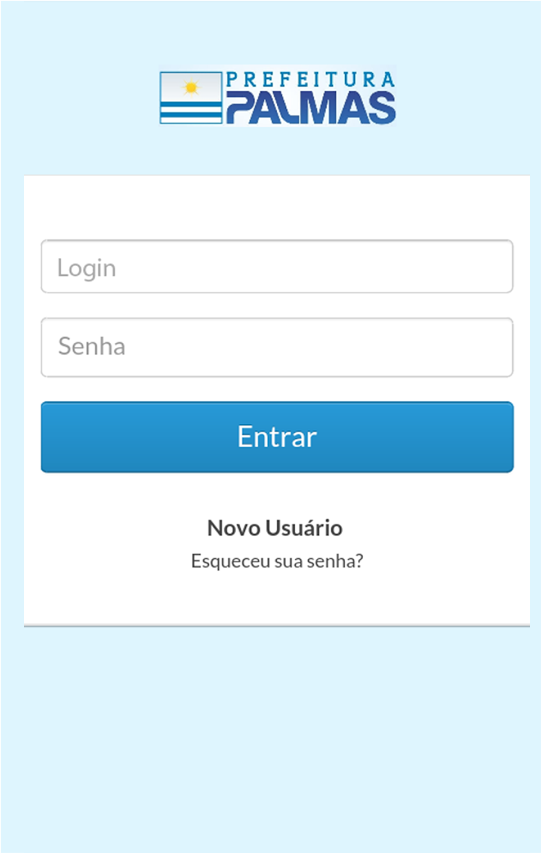
\includegraphics[width=.40\textwidth]{figuras/login_alopequi.png}  &   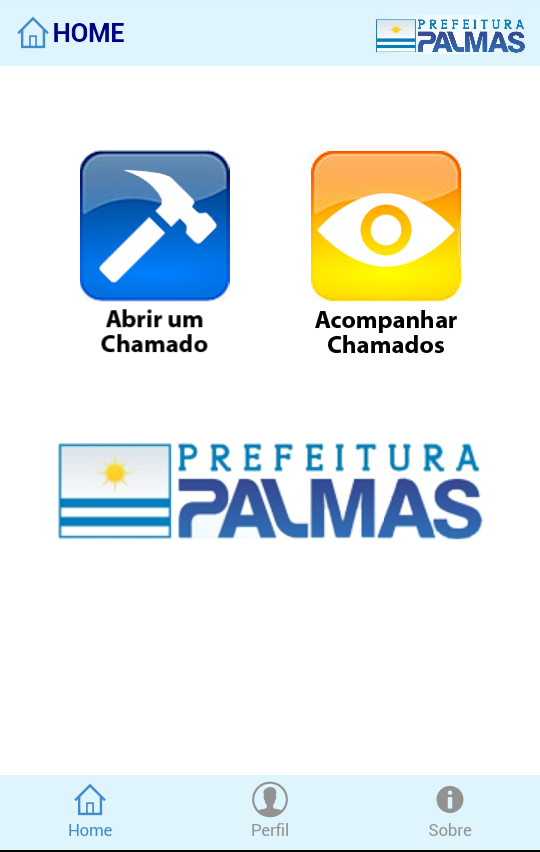
\includegraphics[width=.40\textwidth]{figuras/tela-inicial-alo-pequi.png} 
    \end{tabular}
    \caption{Tela inicial do aplicativo Alô Pequi (Adaptada de \cite{alo_pequi}).}
    \label{alo-pequi}
\end{figure}

Ao utilizar o aplicativo foram constatados diversos pontos positivos e negativos com respeito a usabilidade do sistema, abaixo são relatadas as experiências obtidas com o uso deste:

\subsection*{Pontos Positivos}

\begin{itemize}
    \item Aplicativo muti-plataforma pois utiliza o modelo híbrido de desenvolvimento;
    \item Detecção automática do local do problema pela localização do \acrshort{gps};
    \item Possibilidade de envio de foto do problema; e
    \item Acompanhamento do andamento do chamado.
\end{itemize}

\subsection*{Pontos Negativos}

\begin{itemize}
    \item Aplicativo apresenta lentidão por conta do seu modelo híbrido de desenvolvimento;
    \item Falta a opção de selecionar o local manualmente no mapa;
    \item Falhas na localização pelo \acrshort{gps}; e
    \item Interface muito simples e com poucas funcionalidades.
\end{itemize}

\subsection{Colab}

\noindent O aplicativo Colab é uma rede social que consiste em um sistema de colaboração sobre os problemas de infraestrutura de vários municípios do país, sua utilização atualmente está sendo feita pelas prefeituras de Niterói, Curitiba, Porto Alegre, Santos dentre outras. Existe a possibilidade de uso em qualquer cidade do país mas as ocorrências feitas pelo aplicativo não serão encaminhadas para as prefeituras que não estejam vinculadas à plataforma.

A Figura \ref{colab-app} mostra a tela inicial do aplicativo em que constata-se, pelo fato do sistema se basear no conceito de redes sociais, assim como o \textit{Facebook}\footnote{Facebook: http://www.facebook.com}, algumas características foram herdadas como: compartilhamento da solicitação feita por usuários da região, botão apoiar e opção de comentário.

\begin{figure}[!h]
\centering
    \begin{tabular}{cc}
     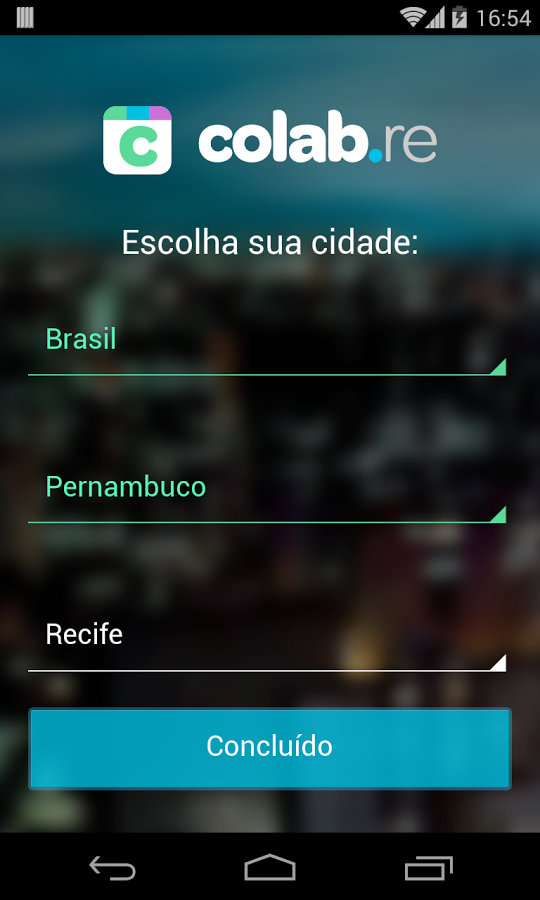
\includegraphics[width=.40\textwidth]{figuras/colab_start.png}  &   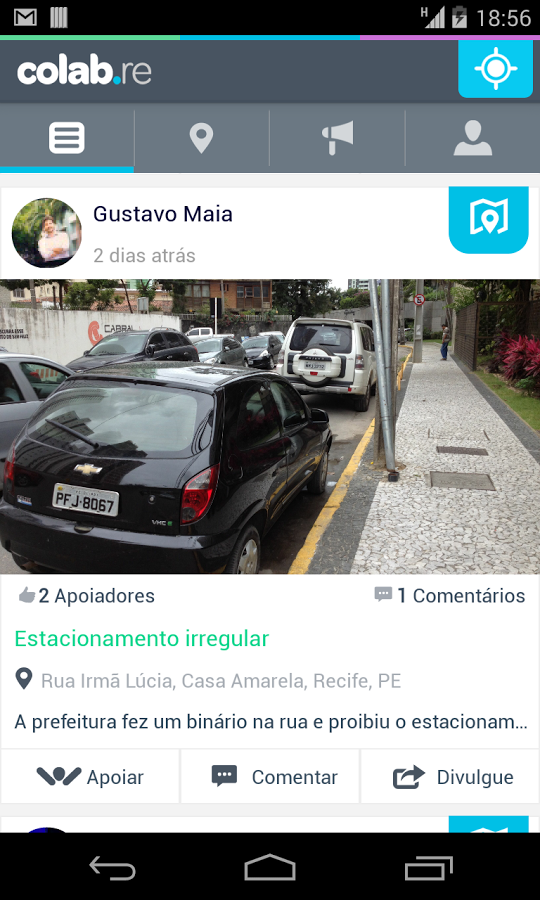
\includegraphics[width=.40\textwidth]{figuras/tela-inicial-colab-re.png} 
    \end{tabular}
    \caption{Tela inicial do aplicativo Colab (Adaptada de \cite{colab}).}
    \label{colab-app}
\end{figure}

Ao utilizar o aplicativo foram observados diversos pontos positivos e negativos com relação à usabilidade do sistema que serão relatados abaixo:

\subsection*{Pontos Positivos}

\begin{itemize}
    \item Padrão de rede social que proporciona um modelo melhor de colaboração;
    \item Opção ``apoiar problema relatado'';
    \item Utilização do \textit{Google Maps} para mostrar uma visão geral dos problemas da cidade;
    \item Disponibilidade de uma opção \textit{web} para o sistema do aplicativo; e
    \item Compartilhamento da reclamação com outras redes sociais.
\end{itemize}

\subsection*{Pontos Negativos}

\begin{itemize}
    \item Falta de moderação das reclamações postadas;
    \item Problemas com \textit{Spam};
    \item Falta de uma opção manual de escolha do local pelo mapa; e
    \item Cadastro feito apenas através de conta na rede social \textit{Facebook}.
\end{itemize}

\subsection{Vigilante App}

\noindent O aplicativo Vigilante App \cite{vigilante_app} é uma rede social colaborativa que visa tornar as informações sobre a cidade mais acessível aos cidadãos, proporcionando uma rede colaborativa de usuários para o compartilhamento de informações como o monitoramento de ocorrências, publicação de problemas com a infraestrutura da cidade dentre outros. A Figura \ref{vigilante-app} mostra a tela inicial do aplicativo.

\begin{figure}[!h]
\centering
    \begin{tabular}{cc}
     
\includegraphics[width=.40\textwidth]{figuras/start_vigilante_app.png}  &   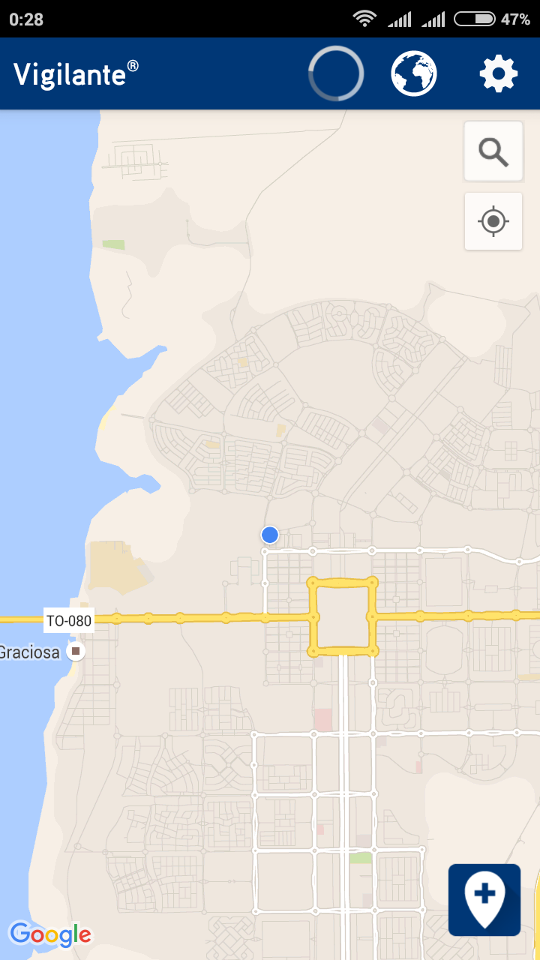
\includegraphics[width=.40\textwidth]{figuras/maps_vigilante.png} 
    \end{tabular}
    \caption{Tela inicial do aplicativo Vigilante App (Adaptada de \cite{vigilante_app}).}
    \label{vigilante-app}
\end{figure}

O sistema atualmente se encontra em fase beta de implantação, mas diversos recursos já estão disponíveis no aplicativo como denúncia de crimes, denúncia de problema infraestruturas como vazamento de água, esgoto e buracos em ruas. Uma característica importante do aplicativo é sua utilização estar voltada totalmente a visualização do mapa da cidade, onde é mostrado uma visão geral sobre os problemas encontrados na cidade. Ao utilizar o aplicativo foram constatados alguns pontos positivos e negativos levando em consideração à facilidade de uso do sistema, abaixo são relatados os pontos identificados:

\subsection*{Pontos Positivos}

\begin{itemize}
    \item Visualização das ocorrências em forma de mapa;
    \item Possibilidade de localização através do \acrshort{gps} ou através da marcação do local no mapa; 
    \item Possibilidade de criação da ocorrência em anonimato e denúncia privada; e
    \item Variedade de categorias para abertura de ocorrências.
\end{itemize}

\subsection*{Pontos Negativos}

\begin{itemize}
    \item Eventuais falhas por conta de estar em fase beta de implantação;
    \item Falta de uma maneira de enumeração das ocorrências em forma de lista de itens; e
    \item Não possibilita o envio de múltiplas fotos ou vídeo.
\end{itemize}

\section{Utilização de prática de  \acrshort{itsm}}

\noindent Em um cenário atual, práticas como o gerenciamento adequado dos ativos de \acrshort{ti} tem sido de grande importância para o sucesso de diversas organizações, motivando os prestadores de serviços uma busca em oferecer serviços de \acrshort{ti} de forma eficaz \cite{introductoryoverviewofitil}. Atualmente, existe uma grande dependência do uso da tecnologia pois ela proporciona aos usuários diversas ferramentas que auxiliam nas tarefas do dia-a-dia.

A \acrshort{ti} tornou-se uma área de influência aos negócios das empresas deixando de ser apenas mais uma ferramenta. A sua utilização tem influenciado as atividades de negócios das organização seja através do uso de ferramentas de escritório ou de \textit{software} que ajuda na tomada de decisão por meio de técnicas de Mineração de Dados. Por esse motivo, a utilização de práticas de gerenciamento de serviços de \acrshort{ti} e governança tornaram-se fundamentais, objetivando promover melhorias no alinhamento dos serviços de \acrshort{ti} com os negócios da organização \cite{servicestrategy, introductoryoverviewofitil}.

O uso de ferramentas de gerenciamento e governança de \acrshort{ti} como o \acrshort{itil} e o \acrshort{cobit} tem como objetivo promover uma melhor gestão dos ativos de \acrshort{ti} e garantir que eles caminhem na mesma direção dos objetivos de negócio da organização \cite{abreu2012implantando}. Atualmente, diversas empresas de nível internacional utilizam práticas de gerenciamento de serviços de \acrshort{ti}, como por exemplo, empresas privadas como a Microsoft\footnote{Microsoft: https://www.microsoft.com}, Walmart\footnote{Walmart: https://www.walmart.com}, organizações financeiras como \textit{Bank of America}\footnote{\textit{Bank of America}: https://www.bankofamerica.com}, pequenas empresas e instituições públicas como departamentos do governo e universidades \cite{albero2010case, arraj2010itil, zhen2007itil}.

O \acrshort{itil} é o \textit{framework} para gerenciamento de serviços de \acrshort{ti} mais utilizado no mundo \cite{servicestrategy, introductoryoverviewofitil, itilbaseditservicemanagementmeasurementsystem}, a aplicação de seus processos tem diversos resultados positivos descritos na literatura como por exemplo, a adoção das práticas do \acrshort{itil} pelo Departamento de Justiça de Ontário  para a criação de um serviço virtual de \textit{help/service desk} em que se obteve excelente resultados, conseguindo economizar cerca de 40\% dos custos de suporte. Outro caso de sucesso foi a empresa Caterpillar que obteve após 18 meses de implantação dos processos do \acrshort{itil} um aumento de 60\% para 90\% do índice de atendimento de incidentes realizado nos acordos de nível de serviço \cite{elephant2004benefits}.

\section{Definição de requisitos para um sistema de Gerenciamento de Incidentes: Um estudo de Caso}

\noindent O artigo Definição de requisitos para um sistema de Gerenciamento de Incidentes: Um estudo de Caso descreve um estudo de caso sobre a definição de requisitos para um sistema de  \gls{ism} de ativos de \textit{software} e \textit{hardware} \cite{jantti2009defining}. O principal objetivo da pesquisa realizada está em buscar maneiras de como examinar os requisitos do sistema de gestão de incidentes, utilizando como base as perspectivas de gerenciamento de serviços de \acrshort{ti} provenientes da biblioteca \acrshort{itil} \cite{jantti2009defining}. O tema de pesquisa do artigo é relevante pois demonstra que os processos de gerenciamento de serviços exigem certas funcionalidades contidas no sistema de \acrshort{ism} que não estão presentes nas ferramentas tradicionais de suporte \cite{jantti2009defining}.

O caso de estudo abordado pelo artigo oferece uma visão geral sobre a implantação de práticas de \acrshort{ism} \cite{jantti2009defining}, onde os conceitos utilizados no artigo são os mesmo adotados em diversas ferramentas de gerenciamento e governança de \acrshort{ti} como o \textit{framework} \acrshort{itil} \cite{introductoryoverviewofitil}, \acrshort{cmmi} \cite{Chrissis:2003:CGP:773274}, \acrshort{cobit} \cite{bernard2012cobit} e o \gls{mof} \cite{pultorak2008mof}. O estudo realizado visa sobre tudo proporcionar uma definição sobre quais tipos de requisitos devem ser levados em consideração para o estabelecimento de um sistema de gerenciamento de incidentes que esteja em acordo com os processos descritos no \acrshort{itil} \cite{introductoryoverviewofitil}. Fornecendo um conjunto de informações sobre quais questões serão levantadas na etapa de especificação dos requisitos \cite{jantti2009defining}.

A metodologia utilizadas no estudo de caso é o \acrshort{itil}, que tem como finalidade servir como guia para a abordagem de gerenciamento de incidentes através da aplicação de um conjunto de melhorias nos processos referentes à gestão dos serviços de \acrshort{ti} \cite{jantti2009defining}. A equipe de pesquisa MaISSI \cite{mailsi} é conhecida por oferecer treinamentos que visam oferecer uma introdução de melhorias nos processos de gestão dos serviços \acrshort{ti}, oferecendo um apoio no desenvolvimento de novos serviços de \textit{software} de alta qualidade além do compartilhamento de novas ideias e experiências \cite{jantti2009defining}.

A organização apresentada no caso de estudo em questão é o departamento do Hospital Universitário de Kuopio na Finlândia, onde foi dado início na etapa de alinhamento das suas operações no início do ano de 2008 através de um serviço de \textit{service desk} oferecido pela Tekplus \cite{jantti2009defining}.

O grupo de desenvolvimento da ferramenta de gerenciamento de incidentes da organização ficou sabendo que a equipe de pesquisa MaISSI dava capacitação para equipes de suporte aos clientes através da criação e descrição dos processos de gerenciamento de incidentes \cite{jantti2009defining}. Foram feitas várias reuniões com o grupo de pesquisa MaISSI com o objetivo em fornecer um conjunto de treinamentos para implantação das práticas do \acrshort{itil} no serviço de \textit{service desk} da organização \cite{jantti2009defining}. Nas reuniões realizadas foram definidas a exigência da inclusão de novos registros dos incidente estejam em concordância com o \gls{sla} estabelecido, fazendo o uso do armazenamento das informações em banco de dados para que haja um gerenciamento efetivo das configurações dos serviços oferecidos pela \acrshort{ti} \cite{jantti2009defining}.

Foram constatado diversos resultados positivos da utilização do \acrshort{itil} no serviço de \textit{help desk} da organização, o que proporcionou uma visão geral sobre a organização e as solicitações de ordem de serviço realizadas pelo sistema \cite{jantti2009defining}. A implantação do \acrshort{itil} na organização promoveu melhorias significativas no controle do sistema de \acrshort{ti}, através das definições presentes nas especificações do \textit{framework}.

\section{\acrshort{ti} e desempenho do gerenciamento de processos de negócios: Estudo de caso da implementação do \acrshort{itil} na indústria de serviços de finanças}

\noindent O artigo \acrshort{ti} e desempenho do gerenciamento de processos de negócios: Estudo de caso da implementação do \acrshort{itil} na indústria de serviços de finanças aborda um caso de estudo da aplicação do gerenciamento de serviços de \acrshort{ti} através da biblioteca \acrshort{itil} no setor financeiro. No trabalho é apontado diversos fatores de sucesso e números sobre a evolução obtidas após a implantação dos processos do \acrshort{itil}. O foco principal do trabalho é apresentar a aplicação das práticas \acrshort{itil} no setor de indústria financeira da Croácia, utilizando como base o ciclo de vida de serviços como apoio para o gerenciamento eficaz dos ativos de \acrshort{ti} \cite{spremic2008and}. A metodologia utilizada como caso de estudo do artigo é referente a implantação das diretrizes das especificações do \acrshort{itil} com apoio de normas internacionais como a ISO 20000 \cite{spremic2008and}.

O caso de estudo apresenta uma análise da evolução dos serviços de \acrshort{ti} prestados por uma empresa croata que está presente no mercado em mais de 100 locais contando com um quadro 5000 funcionários, a empresa oferece serviço financeiro para diversos bancos comerciais da Croácia dentre eles o Banco Nacional Croata \cite{spremic2008and}. Com o aumento significativo da concorrência por empresas menores foi identificado pela a alta administração da empresa a necessidade de uma gestão melhor dos recursos da organização, refletindo assim nos custos operacionais da \acrshort{ti} \cite{spremic2008and}.

A fim de proporcionar um aumento na qualidade dos serviços oferecidos aos clientes, a empresa verificou a necessidade de um melhor gerenciamento dos ativos de \acrshort{ti}. Melhor gestão proporcionada a partir da adoção das práticas \acrshort{itil} e um conjunto de treinamentos que visam tornar o suporte dos serviços de \acrshort{ti} mais proativa frente as necessidades dos clientes \cite{spremic2008and}.

Diversas melhorias foram obtidas pela implantação do \acrshort{itil} na indústria, dentre elas destacasse a redução dos custos operacionais dos serviços proporcionando melhorias na produtividade na prestação de serviços, um aumento significativos na qualidade dos serviços prestados, uma maior satisfação do cliente e a criação de uma abordagem mais profissional em relação aos serviços de tecnologia \cite{spremic2008and}. A seguir são apresentando as tabelas \ref{tbI_itil1}, \ref{tbI_itil2} e \ref{tbI_itil3} que expõem números sobre antes e depois da aplicação das diretrizes do \acrshort{itil} na instituição financeira croata.

\begin{table}[!h]
\centering
\small
\begin{tabular}{|l|c|c|}
\hline
\multicolumn{1}{|c|}{Atividade}                         & Antes do \acrshort{itil}                                                         & Depois do \acrshort{itil}                                                       \\ \hline
Quantidade de problemas graves                          & 22                                                                    & 7                                                                    \\ \hline
Número de problemas repetidos                           & 11                                                                    & 8                                                                    \\ \hline
Tempo médio para descoberta e diagnóstico dos problemas & 4,5 horas                                                             & 3,5 horas                                                            \\ \hline
\% De problemas que foram resolvidos de forma proativa  & \begin{tabular}[c]{@{}c@{}}20\% proativa,\\ 80\% reativa\end{tabular} & \begin{tabular}[c]{@{}c@{}}45\% proativa\\ 55\% reativa\end{tabular} \\ \hline
\end{tabular}
\caption{Ganhos obtidos com a aplicação do \acrshort{itil} no gerenciamento de problemas (Adaptada de \cite{spremic2008and}).}
\label{tbI_itil1}
\end{table}

\begin{table}[!h]
\centering
\small
\begin{tabular}{|l|c|c|}
\hline
\multicolumn{1}{|c|}{Atividade}                                                                                                    & Antes do \acrshort{itil} & Depois do \acrshort{itil} \\ \hline
Tempo médio para a resolução de incidente                                                                                          & 36 min.       & 24 min.        \\ \hline
\begin{tabular}[c]{@{}l@{}}\% do número total de incidentes que foram resolvidos no \\suporte de primeiro nível\end{tabular}      & 18\%          & 37\%           \\ \hline
\begin{tabular}[c]{@{}l@{}}\% do número total de incidentes que tem \\grande impacto sobre serviços\end{tabular}                  & 22\%          & 37\%           \\ \hline
\begin{tabular}[c]{@{}l@{}}\% do número total de incidentes que foram \\recebidos ao lado do \textit{Service Desk}\end{tabular} & 16\%          & 5\%            \\ \hline
\end{tabular}
\caption{Ganhos obtidos com a aplicação do \acrshort{itil} no Gerenciamento de Incidentes (Adaptada de \cite{spremic2008and}).}
\label{tbI_itil2}
\end{table}

\begin{table}[H]
\centering
\small
\begin{tabular}{|l|c|c|}
\hline
\multicolumn{1}{|c|}{Atividade}                         & Antes do \acrshort{itil} & Depois do \acrshort{itil} \\ \hline
\% de mudanças que foram realizadas, como foi planejado & 25\%          & 80\%           \\ \hline
\% de mudanças liberados mas não foi aprovado           & 10\%          & 95\%           \\ \hline
\% de mudanças urgentes                                 & 60\%          & 35\%           \\ \hline
\% de alterações sem sucesso realizados                 & 18\%          & 6\%            \\ \hline
\% do \textit{software} uso que não são autorizadas              & 22\%          & 8\%            \\ \hline
\% de lançamentos errados                               & 13\%          & 10\%           \\ \hline
\% dos laçamentos urgentes                              & 32\%          & 20\%           \\ \hline
\end{tabular}
\caption{Ganhos obtidos com a aplicação do \acrshort{itil} no Gerenciamento de Mudanças e Liberação (Adaptada de \cite{spremic2008and}).}
\label{tbI_itil3}
\end{table}